\chapter{Resolución del trabajo}

\bigskip
La planificación del proyecto se realizó al inicio del mismo y luego se fue alterando según las desviaciones que se producían. El inicio del proyecto fue el 1 de Abril, aunque hasta el 1 de Julio se trabajó en él de manera entrecortada y sin profundidad, y la fecha de fin planificada es el 10 de Septiembre. 

Se podrán distinguir varias etapas en el trabajo, que se ven mejor en la siguiente imagen (Figura \ref{fig:gantt_previsto}) de la planificación:

\begin{itemize}
	\item Preparación y análisis: Aquí se hizo un análisis inicial del proyecto, con tecnologías a usar y un estudio más profundo de algunos conceptos vistos en el curso que se abordarían.
	
	\item Desarrollo del algoritmo genético: esta etapa consta de varias partes, ya que primero se trabajó con distintos algoritmos simples, genéticos o que usaban la paralelización a forma de formación y para facilitar un posterior diseño y análisis del algoritmo que se implementará. A medida que se acababa la implementación del algoritmo final, se hicieron pruebas con los resultados de ambas funciones de optimización.
	
	\item Desarrollo del servicio web: también consta de varias etapas. Primero se creo el BackEnd, y como el FrontEnd requería de los resultados del algoritmo, no se desarrolló hasta obtener algún resultado de este. Una vez completadas estas partes, se pasa al despliegue con una versión estable.
	
	\item Documentación: Aunque se ha ido preparando y almacenando información y recursos durante todo el trascurso del trabajo, la mayor parte de la memoria del trabajo se crea y se plasma en este documento en la etapa final, haciendo las correcciones y mejoras pertinentes.
\end{itemize}
 




\newpage
\section{Planificación}

A continuación se muestra mediante un diagrama de Gantt la planificación estimada del trabajo.

\bigskip
\begin{figure}[h]
	\centering
	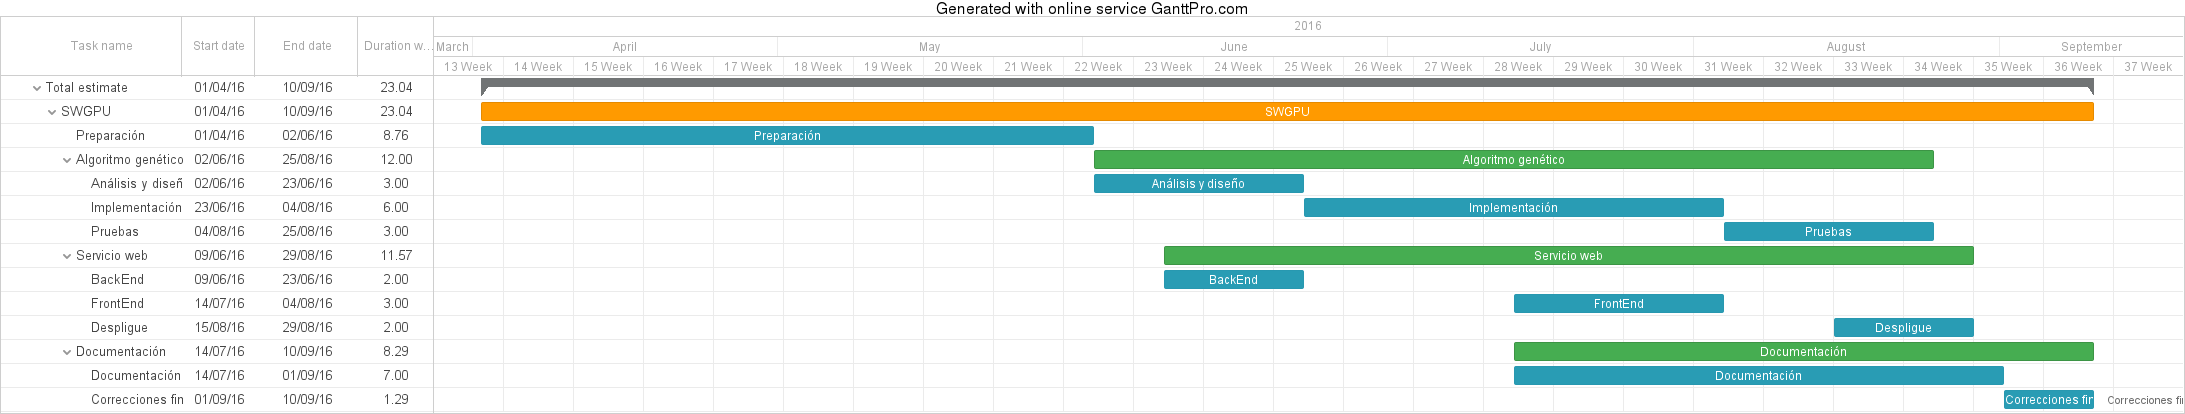
\includegraphics[width=1.0\linewidth]{../images/gantt_prevista}
	\caption[Diagrama Gantt de la planificación prevista del trabajo]{Diagrama Gantt de la planificación prevista del trabajo}
	\label{fig:gantt_previsto}
\end{figure}

\bigskip
Y en la siguiente figura se ve el desarrollo que se a producido, tras desviaciones imprevistas o ajustes de tiempo durante el mismo proceso:


(aproximación del diagrama de Gantt, pendiente la definitiva:)


\bigskip
\begin{figure}[h]
	\centering
	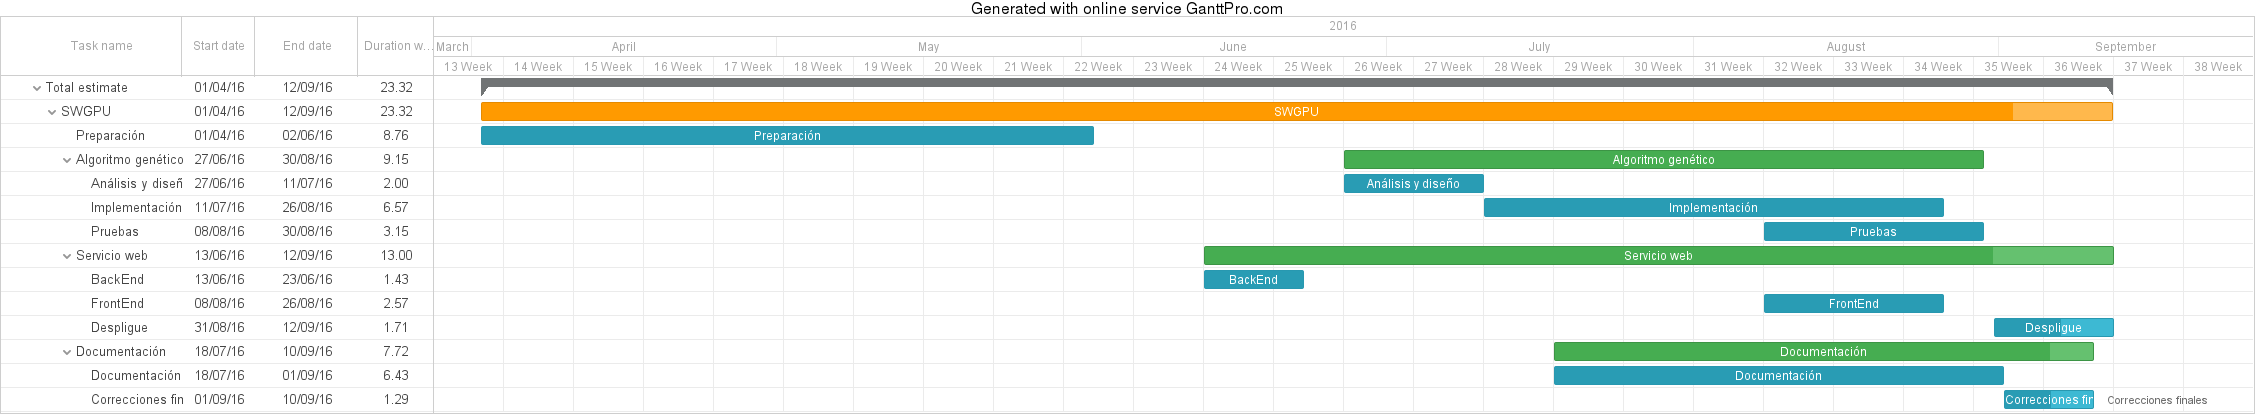
\includegraphics[width=1.0\linewidth]{../images/gantt}
	\caption[Diagrama Gantt de la planificación del trabajo]{Diagrama Gantt de la planificación del trabajo}
	\label{fig:gantt}
\end{figure}


\bigskip
\subsection{Conteo de horas y presupuesto}
\bigskip

\textbf{Conteo de horas}

\begin{itemize}
	
	\item Estimado
		\begin{itemize}
			\item Preparación: 
	
			8.75 semanas, a 3 días/semana, a 2 horas/día: 52.5 horas	
			
			\item Desarrollo de algoritmo genético: 
			
			12 semanas, a 4 días/semana, a 4 horas/día:  192 horas

			\item Desarrollo de servicio web: 
			
			7 semana, a 5 días/semana, a 2 horas/día: 70 horas
			
			\item Documentación: 
			
			8.29 semanas, a 4 días/semana, a 2 horas/día: 66.3 horas
			
			\bigskip			
			\textbf{Con lo que se sumaría un total de 380.8 horas.}
			
		\end{itemize}
	
	\item Real
		\begin{itemize}
			\item Preparación: 
			
			8.76 semanas, a  3 días/semana, a  2 horas/día:  52.5 horas
			
			\item Desarrollo de algoritmo genético: 
			
			9.15 semanas, a 4 días/semana, a 4 horas/día: 146.4 horas
			
			\item Desarrollo de servicio web: 
			
			?? semanas, a 5 días/semana, a 2 horas/día:  ?? horas
			
			\item Documentación: 
			
			?? semanas, a 4 días/semana, a 2 horas/día: ?? horas
			
			\bigskip			
			\textbf{Sumando finalmente un total de ?? horas.}

		\end{itemize}
		
\end{itemize}

\bigskip
\textbf{Presupuesto}

En este punto veremos los presupuesto según el conteo de horas para cada una de las 2 estimaciones y los servicios que requiramos. Suponiendo la media actual de un programador Junior \cite{sueldos}: 9\officialeuro/hora


\bigskip
\begin{itemize}
	
	\item Estimado
	\begin{itemize}
		\item Preparación: 
		
		52.5 horas x 9\officialeuro/hora : 472,5\officialeuro
		
		\item Desarrollo de algoritmo genético: 
		
		192 horas x 9\officialeuro/hora: 1728\officialeuro
		
		\item Desarrollo de servicio web
		
		70 horas x 9\officialeuro/hora: 630\officialeuro
		
		\item Documentación: 

		66.3 horas x 9\officialeuro/hora: 596,7\officialeuro
		
		\item \textit{Instancia que permita usar CUDA}
		
		Se contratarán servicios externos de cómputo mediante CUDA \cite{amazoncuda} con un coste de 1.88\officialeuro/h (2.10\textdollar/h). Suponiendo que este servicio estuviese en total disponibilidad (24 horas los 7 días de la semana) alcanzaría en sólo un mes de servicio los 315,84\officialeuro.
		
		\item \textit{Dominio para alojar una web publica del servicio}
		
		En caso de que no fuese posible, se contrataría un dominio por precios de 2.08\officialeuro a 4.95\officialeuro al mes (con permanencia de 12 meses, en las webs de alojamiento \textit{Hostpapa.es} \cite{hostpapa} y \textit{Dondominio.com} \cite{dondominio})
		
		\bigskip
		\textbf{Presupuesto total estimado: 3745,12\officialeuro (para el desarrollo y sólo un mes en producción) }
		
	\end{itemize}
	
	\item Real
	\begin{itemize}
		\item Preparación
		
		52.5 horas 9\officialeuro/hora
		
		\item Desarrollo de algoritmo genético
		
		146.4 horas 9\officialeuro/hora
		
		\item Desarrollo de servicio web
		
		?? x 9\officialeuro/hora
		
		\item Documentación

		?? x 9\officialeuro/hora
		
		\item \textit{Instancia que permita usar CUDA}
		
		En esta parte se aprovechará el servidor que ofrece la tutora del trabajo {\tutor}, con gran capacidad de cómputo y de manera gratuita. Esto ayudará de manera muy importante al trabajo, ya que reducirá de manera muy importante el presupuesto final del proyecto.
		
		\item \textit{Dominio para alojar una web publica del servicio}
		
		Al igual que en el punto anterior, se aprovechará el servicio de la tutora para lanzar el servicio web, reduciendo también el presupuesto final.
		
		\bigskip
		\textbf{Presupuesto total real: ? \officialeuro}
		
	\end{itemize}

\end{itemize}



\newpage
\section{Tecnologías}

En este apartado se describirán las tecnologías utilizadas en el trabajo. Se desglosarán después de listarlas:

\bigskip
En la parte del servidor:
\begin{itemize}
	\item Python
	\item Django
	\item Apache
	\item C++
	\item CUDA
\end{itemize}

Y de cara al cliente:
\begin{itemize}
	\item HTML5
	\item CSS3
	\item JavaScript
	\item AngularJS
	\item jQuery
	\item JSON
	\item HTML5UP
\end{itemize}

\bigskip
\subsection{Servidor}
\bigskip

\begin{itemize}
	\item \textbf{Python}
	
		Versión usada: 2.7.6
		
		Python \cite{python} es un lenguaje de programación interpretado cuya filosofía hace hincapié en una sintaxis que favorezca un código legible, además de simple y versátil.
				
		\bigskip
		\begin{figure}[h]
			\centering
			
\includegraphics[width=0.2\linewidth]{../images/python}
			\caption[Logo de Python]{Logo de Python}
			\label{fig:pythonlogo}
		\end{figure}
		
		Se trata de un lenguaje de programación multiparadigma, ya que soporta orientación a objetos, programación imperativa y, en menor medida, programación funcional. Es un lenguaje interpretado, usa tipado dinámico y es multiplataforma.
		
	\item \textbf{Django}
	
		Versión usada: 1.10
		
		Django \cite{django} es un framework de alto nivel web de Python. Fomenta el rápido desarrollo y un diseño limpio y pragmático. Se encarga de facilitar la creación de aplicaciones web complejas, ofreciendo las funcionalidades básicas y más útiles al desarrollador, para que pueda centrarse en la escritura de su aplicación.
		
		\bigskip
		\begin{figure}[h]
			\centering
			
\includegraphics[width=0.3\linewidth]{../images/djangologo}
			\caption[Logo de Django]{Logo de Django}
			\label{fig:djangologo}
		\end{figure}
				
	\item Apache
	
		Versión usada: 2.4.12
		
		El servidor HTTP Apache \cite{apache} es un servidor web de código abierto, multiplataforma, extensible y modular. Además, al ser tan popular tiene un gran soporte de la comunidad.
		
		Implementa el protocolo HTTP y la noción de sitio virtual. 
		

		\bigskip
		\begin{figure}[h]
			\centering
			
\includegraphics[width=0.4\linewidth]{../images/apachelogo}
			\caption[Logo de Apache]{Logo de Apache}
			\label{fig:apachelogo}
		\end{figure}
				
	\item \textbf{C++}
	
	Versión usada: 4.8.8
	
	C++ \cite{cpp} es un lenguaje de programación que extiende a C añadiendo mecanismos que permiten la manipulación de objetos. 
	
	Tiene las facilidades de programación genérica junto a los paradigmas de programación estructurada y programación orientada a objetos. 
		 
	
	\item \textbf{CUDA}
	
	Versión usada: 7.5
	
	CUDA \cite{nvidiacuda} es una arquitectura de cálculo paralelo de NVIDIA que aprovecha la gran potencia de la GPU (unidad de procesamiento gráfico) para proporcionar un incremento extraordinario del rendimiento del sistema.
	
	Dispone de una gran comunidad, ya que es la arquitectura de cálculo paralelo más usada en la actualidad, en parte gracias a su potencia y la facilidad de uso para los desarrolladores.

	
	La plataforma de cálculo paralelo CUDA proporciona unas cuantas extensiones de C y C++ que permiten implementar el paralelismo en el procesamiento de tareas y datos con diferentes niveles de granularidad y con la flexibilidad de usar varios lenguajes, como son C, C++ y Fortran. 
	
	Dispone de numerosas facilidades para los desarrolladores, como herramientas de desarrollo, documentación y su \textit{toolkit}.

		\bigskip
		\begin{figure}[h]
			\centering
			
\includegraphics[width=0.3\linewidth]{../images/cudalogo}
			\caption[Logo de CUDA]{Logo de CUDA}
			\label{fig:cudalogo}
		\end{figure}
	
			
\end{itemize}
	

\newpage
\subsection{Cliente}
\bigskip


\begin{itemize}
	\item \textbf{HTML5}
	
	HTML (HyperText Markup Language) \cite{html} en su la quinta revisión, es el lenguaje básico de la World Wide Web. Es un estándar que sirve de referencia de elaboración de páginas web en sus diferente versiones. Define una estructura básica y un código para la definición de contenido de una página web, como texto, imágenes o vídeos. Usa un sistema para formatear el layout de nuestras páginas, así como hacer algunos ajustes a su aspecto. Los navegadores como Chrome, Firefox, Explorer o Safari puede saber como representar el contenido de una web, con las ubicaciones de todos los elementos.
	
	
	\bigskip
	\begin{figure}[h]
		\centering
		
\includegraphics[width=0.3\linewidth]{../images/htmllogo}
		\caption[Logo de HTML5]{Logo de HTML5}
		\label{fig:htmllogo}
	\end{figure}
	
	\item \textbf{CSS3}
		
	 CSS (Cascading Style Sheets) \cite{css} u hoja de estilo en cascada, es un lenguaje usado para definir y crear la presentación de un documento estructurado escrito en HTML o XML2. El World Wide Web Consortium (W3C) es el encargado de formular la especificación de las hojas de estilo, al igual que del lenguaje HTML, que servirán de estándar para los agentes de usuario o navegadores.

	 Aunque la información de estilo puede ser definida en el mismo documento HTML, la idea que se encuentra detrás del desarrollo de CSS es separar la estructura de un documento de su presentación. 

	
	\bigskip
	\begin{figure}[h]
		\centering
		
\includegraphics[width=0.3\linewidth]{../images/csslogo}
		\caption[Logo de CSS3]{Logo de CSS3}
		\label{fig:csslogo}
	\end{figure}
		
	\item \textbf{JavaScript}
		
	JavaScript \cite{js} es un lenguaje de programación interpretado, que se define como orientado a objetos, basado en prototipos, imperativo, débilmente tipado y dinámico.

	Se utiliza principalmente en su forma del lado del cliente, implementado como parte de un navegador web permitiendo mejoras en la interfaz de usuario y páginas web dinámicas (aunque existe una forma de JavaScript del lado del servidor). 

	Todos los navegadores modernos interpretan el código JavaScript integrado en las páginas web. Para interactuar con una página web se provee al lenguaje JavaScript de una implementación del Document Object Model (DOM).

	\bigskip
	\begin{figure}[h]
		\centering
		
\includegraphics[width=0.3\linewidth]{../images/jslogo}
		\caption[Logo de JavasSript]{Logo de JavaScript}
		\label{fig:jslogo}
	\end{figure}
			
	\item \textbf{AngularJS}
		
	Versión usada: 1.5.7
		
	AngularJS \cite{angularjs} es un framework de JavaScript de código abierto, mantenido por Google, que se utiliza para crear y mantener aplicaciones web de una sola página. Su objetivo es aumentar las aplicaciones basadas en navegador con capacidad de Modelo Vista Whatever (MVW), en un esfuerzo para hacer que el desarrollo y las pruebas sean más fáciles.

	La biblioteca lee el HTML que contiene atributos de las etiquetas personalizadas adicionales, entonces obedece a las directivas de los atributos personalizados, y une las piezas de entrada o salida de la página a un modelo representado por las variables estándar de JavaScript, que además se pueden configurar manualmente, o recuperados de los recursos JSON estáticos o dinámico

	\bigskip
	\begin{figure}[h]
		\centering
		
\includegraphics[width=0.4\linewidth]{../images/angularjslogo}
		\caption[Logo de AngularJS]{Logo de AngularJS}
		\label{fig:angularjslogo}
	\end{figure}
		
	\item \textbf{jQuery}
	
		Versión usada: 1.11.3
		
	jQuery \cite{jquery} es una biblioteca de JavaScript que permite simplificar la manera de interactuar con los documentos HTML, manipular el árbol DOM, manejar eventos, desarrollar animaciones y agregar interacción con la técnica AJAX a páginas web.

	jQuery, al igual que otras bibliotecas, ofrece una serie de funcionalidades basadas en JavaScript de manera muy reducida, por lo que con las funciones propias de esta biblioteca se logran grandes resultados en menos tiempo y espacio. Todo esto hace que sea la biblioteca JavaScript más usada.
		
	\bigskip
	\begin{figure}[h]
		\centering
		
\includegraphics[width=0.4\linewidth]{../images/jquerylogo}
		\caption[Logo de jQuery]{Logo de jAuery}
		\label{fig:jquerylogo}
	\end{figure}
		
	\item \textbf{JSON}
		
	JSON (JavaScript Object Notation) \cite{json} es un formato ligero de intercambio de datos. Gracias a su sencillez es fácil leerlo y escribirlo para humanos, mientras que para las máquinas es simple interpretarlo y generarlo.
	
	Es un formato de texto que es completamente independiente del lenguaje pero utiliza convenciones que son ampliamente conocidos por los programadores de los principales lenguajes. 
	
	Estas propiedades hacen que JSON sea un lenguaje ideal para el intercambio de datos.

	\bigskip
	\begin{figure}[h]
		\centering
		
\includegraphics[width=0.3\linewidth]{../images/jsonlogo}
		\caption[Logo de JSON]{Logo de JSON}
		\label{fig:jsonlogo}
	\end{figure}
	
	\item \textbf{HTML5UP}
		
	HTML5UP \cite{htmlup} Web con múltiples plantillas disponibles (usando HTML y JavaScript) y estilos CSS con los que crear la estructura básica de proyectos web. Son completamente personalizables y	tienen un diseño web adaptable (\textit{responsive}) de manera que la web que creemos se adaptará a cualquier pantalla, punto muy importante en la actualidad, debido a la multitud de dispositivos y tamaños de pantalla que existen.

	\bigskip
	\begin{figure}[h]
		\centering
		
\includegraphics[width=0.3\linewidth]{../images/htmluplogo}
		\caption[Logo de HTML5UP]{Logo de HTML5UP}
		\label{fig:htmluplogo}
	\end{figure}
		
\end{itemize}
	
	
	

\newpage
\section{Herramientas}

En este apartado se listarán y desglosarán las herramientas usadas para usar las tecnologías anteriores.


\begin{itemize}
	\item \textbf{Nsight Eclipse Edition}
	
	Versión usada: 7.5
		
	Nsigh (NVIDIA Nsight Eclipse Edition) \cite{nsight} es la gran plataforma de desarrollo para cálculo heterogéneo. Permite trabajar con potentes herramientas de depuración y análisis del rendimiento para optimizar el funcionamiento de la CPU y la GPU. Esta plataforma permite optimizar el rendimiento de manera intuitiva, identificar y analizar los cuellos de botella y observar el comportamiento de todas las actividades del sistema.

	Consta de varias plantillas y ejemplos, además de estar disponible varios sistemas operativos.
 
	\bigskip
	\begin{figure}[h]
		\centering
		
\includegraphics[width=0.5\linewidth]{../images/nsightlogo}
		\caption[Logo de Nsight]{Logo de Nsight}
		\label{fig:nsightlogo}
	\end{figure}
	
	\item \textbf{TeXstudio}
		
		Versión usada: 2.11.0
		
	TeXstudio \cite{texstudio} es un entorno de escritura para la creación de documentos LaTeX de manera fácil, cómoda e intuitiva. Tiene numerosas características, como el resaltado de sintaxis, pre-visualizador integrado, verificación de referencias y varios asistentes. 

	Tiene una gran documentación y comunidad, además de estar disponible para los sistemas operativos más importantes.
		
	\bigskip
	\begin{figure}[h]
		\centering
		
\includegraphics[width=0.3\linewidth]{../images/texstudiologo}
		\caption[Logo de TeXstudio]{Logo de TeXstudio}
		\label{fig:texstudiologo}
	\end{figure}
			
	\item \textbf{Git}
			
		Versión usada: 1.91
		
	Git \cite{git} es un software de control de versiones, pensando en la eficiencia y la confiabilidad del mantenimiento de versiones de aplicaciones cuando éstas tienen un gran número de archivos de código fuente. 

	Git se considera un sistema de control de versiones con funcionalidad plena y con multitud de características, como la gestión distribuida o la rápida gestión de ramas. 

	\bigskip
	\begin{figure}[h]
		\centering
		
\includegraphics[width=0.3\linewidth]{../images/gitlogo}
		\caption[Logo de Git]{Logo de Git}
		\label{fig:gitlogo}
	\end{figure}
				
	\item \textbf{Sublime Text}
			
	Versión usada: 2, versión de evaluación
		
	Sublime Text \cite{sublimetext} es un editor de texto y de código fuente. Originalmente fue desarrollado como una extensión de Vim y con el tiempo fue creando una identidad propia.

	Poseee varias características para los desarrolladores, como un \textit{minimapa} del código, multi-selección y multi-cursor, búsqueda dinámica y soporte a multitud de lenguajes.


	\bigskip
	\begin{figure}[h]
		\centering
		
\includegraphics[width=0.3\linewidth]{../images/sublimetextlogo}
		\caption[Logo de Sublime Text]{Logo de Sublime Text}
		\label{fig:sublimetextlogo}
	\end{figure}
				
	\item \textbf{Gimp}
			
	Versión usada: 2.8.10
		
	GIMP (GNU Image Manipulation Program) \cite{gimp} es un programa de edición de imágenes digitales en forma de mapa de bits, tanto dibujos como fotografías. 

	Tiene multitud de herramientas para el retoque y edición de imágenes o un dibujo libre.

	Esta disponible para la mayoría de los sistemas operativos y en varios lenguajes.

	\bigskip
	\begin{figure}[h]
		\centering
		
\includegraphics[width=0.3\linewidth]{../images/gimplogo}
		\caption[Logo de Gimp]{Logo de Gimp}
		\label{fig:gimplogo}
	\end{figure}
	
	
	\item \textbf{GanttPRO}
	
	GanttPRO \cite{ganttpro} permite la gestión de proyectos mediante diagramas de Gantt.

	Mediante su interfaz se pude planificar y gestionar proyectos con facilidad con diagramas de Gantt, mediante tareas, subtareas o duraciones dinámicas. 	

	\bigskip
	\begin{figure}[h]
		\centering
		
\includegraphics[width=0.3\linewidth]{../images/ganttprologo}
		\caption[Logo de GanttPRO]{Logo de GanttPRO}
		\label{fig:ganttprologo}
	\end{figure}

	\item \textbf{Draw.io}
	
	Draw.io \cite{drawioweb} es una herramienta para crear varios tipos de diagramas, entre ellos del tipo UML.
	
	\bigskip
	\begin{figure}[h]
		\centering
		
\includegraphics[width=0.3\linewidth]{../images/drawiologo}
		\caption[Logo de Draw.io]{Logo de Draw.io}
		\label{fig:drawiologo}
	\end{figure}
					
\end{itemize}

